\documentclass[conference]{IEEEtran}
\IEEEoverridecommandlockouts

\usepackage{cite}
\usepackage{amsmath,amssymb,amsfonts}
\usepackage{algorithm}
\usepackage{algpseudocode}
\usepackage{graphicx}
\usepackage{textcomp}
\usepackage{xcolor}
\usepackage{booktabs}
\usepackage{multirow}
\usepackage{array}
\usepackage{tikz}
\usepackage{pgfplots}
\pgfplotsset{compat=1.18}
\usetikzlibrary{shapes.geometric, arrows.meta, positioning, calc, fit, backgrounds, matrix}
\usepackage[hidelinks]{hyperref}

\definecolor{ieeeBlue}{RGB}{0, 98, 155}
\definecolor{claheOrange}{RGB}{217, 95, 2}
\definecolor{cmHigh}{RGB}{8, 81, 156}
\definecolor{cmMedHigh}{RGB}{49, 130, 189}
\definecolor{cmMed}{RGB}{107, 174, 214}
\definecolor{cmLow}{RGB}{189, 215, 231}
\definecolor{cmVeryLow}{RGB}{239, 243, 255}

\begin{document}

\title{Lightweight Brain Tumor MRI Classification Using HOG Features, PCA, and Class-Weighted SVM: A Reproduction and CLAHE Enhancement Study}

\author{
\IEEEauthorblockN{Yash Goyal}
\IEEEauthorblockA{\textit{Dept. of Computer Science and Engineering}}
\and
\IEEEauthorblockN{Satyarth Chaudhary}
\IEEEauthorblockA{\textit{Dept. of Computer Science and Engineering}}
\and
\IEEEauthorblockN{Manshu Saini}
\IEEEauthorblockA{\textit{Dept. of Computer Science and Engineering}}
}

\maketitle

\begin{abstract}
Automated classification of brain tumors from Magnetic Resonance Imaging (MRI) scans is a vital computer-aided diagnosis task. While deep convolutional neural networks and Vision Transformers achieve high accuracy, their substantial computational overhead, large memory footprint, and reliance on specialized GPU hardware often limit deployment in resource-constrained clinical settings. Recently, Warsito \emph{et al.} (2026) proposed an ultra-lightweight classification pipeline combining $16 \times 16$ spatial downsampling, Histogram of Oriented Gradients (HOG) feature extraction, Principal Component Analysis (PCA), and class-weighted Support Vector Machines (SVMs). In this work, we conduct a rigorous, leakage-free reproduction of this lightweight paradigm on the four-class Kaggle Brain Tumor MRI dataset ($3,264$ scans across \emph{glioma}, \emph{meningioma}, \emph{pituitary tumor}, and \emph{no tumor}) and propose a targeted preprocessing extension: full-resolution Contrast Limited Adaptive Histogram Equalization (CLAHE) prior to spatial downsampling. Because shrinking an MRI slice directly to $16 \times 16$ discards fine anatomical textures, applying CLAHE at native resolution amplifies local tissue boundaries before interpolation so that edge gradients carry greater discriminative weight in the low-resolution HOG representation. Across seven evaluated SVM configurations, the degree-4 Polynomial SVM ($C=10$) achieves the highest overall performance, reaching $86.04\%$ test accuracy ($95\%$ bootstrap CI: $82.5\%\text{--}89.3\%$), $90.17\%$ weighted precision, $84.73\%$ weighted F1-score, and a macro one-vs-rest ROC-AUC of $0.9817$, with a total training time of $1.88\text{ s}$ and an inference latency of $0.43\text{ ms}$ per MRI scan on CPU. Furthermore, our CLAHE extension improves the cross-validated GridSearch RBF SVM by $+3.05\%$ in accuracy ($74.87\% \rightarrow 77.92\%$) and $+3.65\%$ in weighted F1-score ($69.82\% \rightarrow 73.47\%$), while improving the macro ROC-AUC of the class-weighted Polynomial SVM from $0.9412$ to $0.9471$. Finally, we provide an in-depth mathematical and empirical analysis uncovering how post-HOG intensity scaling interacts with SVM kernel parameterization and class-specific recall trade-offs between glioma and pituitary tumors.
\end{abstract}

\begin{IEEEkeywords}
Brain Tumor Classification, Magnetic Resonance Imaging (MRI), Histogram of Oriented Gradients (HOG), Principal Component Analysis (PCA), Support Vector Machine (SVM), Contrast Limited Adaptive Histogram Equalization (CLAHE), Cost-Sensitive Learning, Lightweight Computer Vision.
\end{IEEEkeywords}

\section{Introduction}
Brain tumors represent one of the most life-threatening neurological disorders, characterized by the abnormal and uncontrolled proliferation of cells within the cranial cavity. Among primary intracranial neoplasms, \emph{gliomas} arise from glial support cells and account for the majority of malignant brain tumors; \emph{meningiomas} originate in the meningeal membranes enveloping the brain and spinal cord; and \emph{pituitary adenomas} develop within the pituitary gland at the base of the brain, frequently causing endocrine dysfunction and visual field defects \cite{cheng2015enhanced}. Early and accurate differentiation among these tumor subtypes, as well as reliable distinction from healthy brain anatomy (\emph{no tumor}), is critical for treatment planning, surgical resection strategy, and prognosis assessment.

Magnetic Resonance Imaging (MRI) is the clinical gold standard for non-invasive neuroimaging due to its superior soft-tissue contrast and absence of ionizing radiation. However, manual interpretation of multi-planar MRI slices (axial, coronal, and sagittal views) is time-consuming and subject to inter-observer variability among radiologists. Over the past decade, deep learning architectures such as Convolutional Neural Networks (CNNs) \cite{deepak2019brain, sultan2019multi} and Vision Transformers (ViTs) \cite{tummala2022classification} have dominated automated brain tumor classification. Despite their diagnostic accuracy, deep architectures typically contain millions of trainable parameters, require gigabytes of memory, and depend on GPU acceleration for training and real-time inference. In rural clinics, portable diagnostic stations, and developing healthcare infrastructures, computationally lightweight algorithms that execute rapidly on standard CPU hardware remain highly desirable.

Addressing this need, Warsito \emph{et al.} \cite{warsito2026lightweight} recently introduced a lightweight brain tumor classification framework in the \emph{Journal of Applied Data Sciences} (2026). Their pipeline resizes grayscale MRI scans to $16 \times 16$ pixels, extracts dense Histogram of Oriented Gradients (HOG) descriptors \cite{dalal2005histograms}, applies Principal Component Analysis (PCA) retaining $98\%$ variance, and trains Support Vector Machines (SVMs) \cite{cortes1995support} with custom class weights to handle dataset imbalance.

While downsampling MRI scans to $16 \times 16$ pixels enables sub-second training and sub-millisecond inference, we observe a fundamental signal-processing limitation in the baseline pipeline: direct spatial downsampling acts as a strong low-pass filter that averages out subtle soft-tissue intensity transitions, peritumoral edema boundaries, and sulcal contours. If local contrast in the original MRI slice is low, critical morphological gradients vanish before the HOG operator is ever applied. To mitigate this information loss without increasing the downstream feature dimensionality or classifier complexity, we propose applying \textbf{Contrast Limited Adaptive Histogram Equalization (CLAHE)} \cite{zuiderveld1994contrast} at full native spatial resolution \emph{prior} to $16 \times 16$ downsampling.

The primary contributions of this project are summarized as follows:
\begin{enumerate}
    \item \textbf{End-to-End Reproduction and Verification:} We implement a modular, strictly leakage-free reproduction of Warsito \emph{et al.} \cite{warsito2026lightweight} on the 3,264-image Kaggle Brain Tumor MRI dataset \cite{bhuvaji2020brain}, evaluating seven SVM configurations including 5-fold cross-validated grid search across 52 hyperparameter combinations.
    \item \textbf{Full-Resolution CLAHE Preprocessing Extension:} We design and evaluate a pre-downsampling CLAHE enhancement stage ($\text{clipLimit}=2.0$, $8 \times 8$ tile grid) that amplifies local anatomical boundaries at native resolution before spatial compression to $16 \times 16$.
    \item \textbf{Rigorous Statistical Evaluation:} Beyond point estimates of accuracy, precision, recall, and F1-score, we incorporate 1,000-round non-parametric bootstrap $95\%$ confidence intervals, macro one-vs-rest ROC-AUC from continuous SVM decision functions, and class-wise confusion matrix diagnostics.
    \item \textbf{Theoretical and Empirical Failure-Mode Analysis:} We mathematically explain two counter-intuitive behaviors in the baseline paper's specification: (a) why the post-HOG division by $255.0$ causes default Linear SVMs ($C=1.0$) to collapse to a majority-class predictor ($18.78\%$ accuracy) while adaptive $\gamma_{\text{scale}}$ kernels remain unaffected, and (b) the sharp sensitivity trade-off between \emph{glioma} and \emph{pituitary} recall across degree-3 and degree-4 polynomial kernels.
\end{enumerate}

\section{Related Work}

\subsection{Classical Feature Engineering in Brain MRI}
Traditional computer-aided diagnosis (CAD) systems for brain MRI rely on handcrafted texture, shape, and gradient descriptors paired with shallow classifiers. Gray-Level Co-occurrence Matrices (GLCM) \cite{haralick1973textural}, Discrete Wavelet Transforms (DWT) \cite{chaplot2006classification}, Gabor filter banks, and Local Binary Patterns (LBP) have been widely employed to capture tissue heterogeneity. Cheng \emph{et al.} \cite{cheng2015enhanced} demonstrated that augmenting tumor region-of-interest (ROI) margins and extracting intensity histograms, GLCM, and Bag-of-Words (BoW) features significantly improved three-class tumor classification. Dalal and Triggs \cite{dalal2005histograms} originally formulated Histogram of Oriented Gradients (HOG) for pedestrian detection, capturing local edge orientation distributions normalized across overlapping spatial blocks. In medical imaging, HOG has proven effective for characterizing structural asymmetries in cranial anatomy and mass lesions when coupled with dimensionality reduction techniques such as PCA \cite{jolliffe2016principal}.

\subsection{Kernel Classifiers and Class-Imbalanced Learning}
Support Vector Machines (SVMs) \cite{cortes1995support} construct maximum-margin hyperplanes in high-dimensional reproducing kernel Hilbert spaces (RKHS) and exhibit strong generalization when the number of features is comparable to the sample size. Because medical datasets frequently suffer from class imbalance, where healthy control scans or specific rare tumor subtypes are underrepresented, standard empirical risk minimization can bias the decision boundary toward majority classes. Cost-sensitive SVMs address this by assigning class-specific penalty weights $C_k = w_k C$ to slack variables \cite{veropoulos1999controlling}. Warsito \emph{et al.} \cite{warsito2026lightweight} combined PCA-reduced HOG vectors with polynomial and RBF SVMs, introducing heuristic class weights to compensate for the minority \emph{no\_tumor} training class.

\subsection{Contrast Enhancement via CLAHE in Neuroimaging}
MRI acquisitions often exhibit intensity non-uniformity, bias fields, and low dynamic range between tumor parenchyma and surrounding gray/white matter. Global Histogram Equalization (GHE) stretches the intensity histogram across the entire image but frequently over-amplifies background noise and saturates bright regions. Adaptive Histogram Equalization (AHE) \cite{pizer1987adaptive} computes local histograms within contextual tiles, and Zuiderveld \cite{zuiderveld1994contrast} refined this approach into Contrast Limited Adaptive Histogram Equalization (CLAHE) by clipping the local histogram at a predefined threshold before computing the cumulative distribution function (CDF). In brain MRI analysis, CLAHE has been shown to sharpen lesion borders and improve segmentation and classification robustness \cite{kaur2018comparison}. In our work, we specifically investigate the role of CLAHE as a \emph{pre-antialiasing contrast booster} prior to extreme spatial downsampling ($16 \times 16$).



\section{Dataset Description}
We conduct all experiments on the publicly available \textbf{Brain Tumor Classification (MRI)} dataset curated by Bhuvaji \emph{et al.} \cite{bhuvaji2020brain}. The dataset comprises $3,264$ two-dimensional grayscale brain MRI slices acquired across axial, coronal, and sagittal planes, pre-partitioned into standard \texttt{Training} ($2,870$ images, $87.93\%$) and \texttt{Testing} ($394$ images, $12.07\%$) directories. Each scan belongs to one of four mutually exclusive diagnostic categories indexed alphabetically as $y \in \{0, 1, 2, 3\}$:
\begin{itemize}
    \item \textbf{Class 0 (\texttt{glioma\_tumor}):} Intra-axial glial neoplasms often exhibiting irregular, infiltrative margins and heterogeneous necrotic cores.
    \item \textbf{Class 1 (\texttt{meningioma\_tumor}):} Extra-axial dural-based masses typically presenting as well-circumscribed, homogeneously enhancing lesions adjacent to the skull or falx.
    \item \textbf{Class 2 (\texttt{no\_tumor}):} Normal brain MRI slices demonstrating intact ventricular symmetry and absence of space-occupying lesions.
    \item \textbf{Class 3 (\texttt{pituitary\_tumor}):} Sellar and suprasellar adenomas localized consistently near the pituitary fossa.
\end{itemize}

\begin{table}[t]
\centering
\caption{Class Distribution of the Brain Tumor MRI Dataset Across Training and Testing Splits, Along with Paper Class Weights}
\label{tab:dataset}
\setlength{\tabcolsep}{4.5pt}
\begin{tabular}{clrrrrrc}
\toprule
\textbf{ID} & \textbf{Class Name} & \textbf{Train} & \textbf{Train \%} & \textbf{Test} & \textbf{Test \%} & \textbf{Total} & \textbf{Weight $w_k$} \\
\midrule
0 & \texttt{glioma\_tumor}     &   826 & 28.78\% & 100 & 25.38\% &   926 & 0.69 \\
1 & \texttt{meningioma\_tumor} &   822 & 28.64\% & 115 & 29.19\% &   937 & 0.69 \\
2 & \texttt{no\_tumor}         &   395 & 13.76\% & 105 & 26.65\% &   500 & 0.90 \\
3 & \texttt{pituitary\_tumor}  &   827 & 28.82\% &  74 & 18.78\% &   901 & 0.60 \\
\midrule
\multicolumn{2}{l}{\textbf{Total}} & \textbf{2,870} & \textbf{100.0\%} & \textbf{394} & \textbf{100.0\%} & \textbf{3,264} & N/A \\
\bottomrule
\end{tabular}
\end{table}

Table~\ref{tab:dataset} details the sample distribution across both splits alongside the custom class weights specified in Section~3.5 of Warsito \emph{et al.} \cite{warsito2026lightweight}. Two structural properties of the dataset merit close attention:
\begin{enumerate}
    \item \textbf{Training Class Imbalance:} In the training split, the three tumor classes are nearly balanced ($826$, $822$, and $827$ samples, respectively), whereas \texttt{no\_tumor} contains only $395$ samples ($13.76\%$, an imbalance ratio of $2.09:1$). This motivated the higher penalty weight $w_2 = 0.90$ for \texttt{no\_tumor}.
    \item \textbf{Prior Shift Between Training and Testing Splits:} While \texttt{no\_tumor} is the smallest class in the training set ($13.76\%$), it constitutes $26.65\%$ ($105/394$) of the test set. Conversely, \texttt{pituitary\_tumor} is the largest class in the training set ($827$ samples, $28.82\%$) but the smallest class in the test set ($74$ samples, $18.78\%$).
\end{enumerate}

\section{Proposed Methodology and System Architecture}

\begin{figure*}[t]
\centering
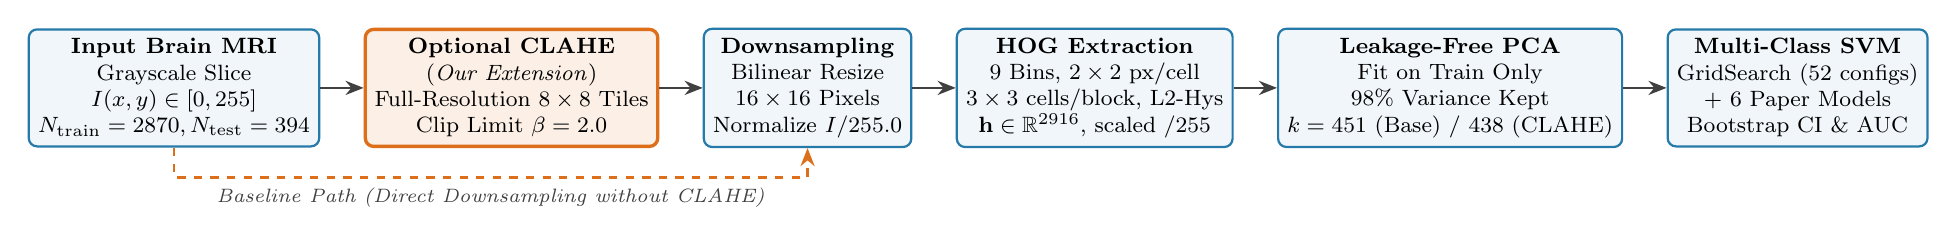
\begin{tikzpicture}[
    node distance=0.45cm and 0.55cm,
    box/.style={rectangle, rounded corners=3pt, draw=ieeeBlue!85, fill=ieeeBlue!6, thick, minimum height=1.25cm, align=center, font=\footnotesize},
    extbox/.style={rectangle, rounded corners=3pt, draw=claheOrange!90, fill=claheOrange!10, very thick, minimum height=1.25cm, align=center, font=\footnotesize},
    arrow/.style={-{Stealth[length=2.3mm, width=1.8mm]}, thick, draw=black!75},
    dashedarrow/.style={-{Stealth[length=2.3mm, width=1.8mm]}, thick, dashed, draw=claheOrange!90}
]

\node[box, minimum width=2.2cm] (input) {\textbf{Input Brain MRI}\\Grayscale Slice\\$I(x,y) \in [0,255]$\\$N_{\text{train}}=2870, N_{\text{test}}=394$};

\node[extbox, right=of input, minimum width=2.45cm] (clahe) {\textbf{Optional CLAHE}\\(\emph{Our Extension})\\Full-Resolution $8\times 8$ Tiles\\$\text{Clip Limit } \beta = 2.0$};

\node[box, right=of clahe, minimum width=2.25cm] (resize) {\textbf{Downsampling}\\Bilinear Resize\\$16 \times 16$ Pixels\\Normalize $I / 255.0$};

\node[box, right=of resize, minimum width=2.55cm] (hog) {\textbf{HOG Extraction}\\9 Bins, $2\times 2$ px/cell\\$3\times 3$ cells/block, L2-Hys\\$\mathbf{h} \in \mathbb{R}^{2916}$, scaled $/255$};

\node[box, right=of hog, minimum width=2.4cm] (pca) {\textbf{Leakage-Free PCA}\\Fit on Train Only\\$98\%$ Variance Kept\\$k=451$ (Base) / $438$ (CLAHE)};

\node[box, right=of pca, minimum width=2.45cm] (svm) {\textbf{Multi-Class SVM}\\GridSearch (52 configs)\\+ 6 Paper Models\\Bootstrap CI \& AUC};

\draw[arrow] (input) -- (clahe);
\draw[arrow] (clahe) -- (resize);
\draw[arrow] (resize) -- (hog);
\draw[arrow] (hog) -- (pca);
\draw[arrow] (pca) -- (svm);

\draw[dashedarrow] (input.south) -- ++(0,-0.38) -| node[pos=0.25, below, font=\scriptsize\itshape, text=black!75] {Baseline Path (Direct Downsampling without CLAHE)} (resize.south);

\end{tikzpicture}
\caption{System architecture of the reproduced baseline pipeline (Warsito \emph{et al.} \cite{warsito2026lightweight}) and our proposed full-resolution CLAHE enhancement extension. PCA is fitted strictly on the training feature matrix $\mathbf{X}_{\text{train}} \in \mathbb{R}^{2870 \times 2916}$ to prevent test-set leakage.}
\label{fig:pipeline}
\end{figure*}

Fig.~\ref{fig:pipeline} illustrates the complete four-stage classification architecture implemented in our codebase (\texttt{features.py}, \texttt{models.py}, \texttt{evaluate.py}, and \texttt{reproduce.py}). Below we formalize each stage mathematically.

\subsection{Image Preprocessing and Full-Resolution CLAHE Extension}
Let $I \in \{0, 1, \dots, 255\}^{H \times W}$ denote an input single-channel grayscale MRI slice loaded via OpenCV (\texttt{cv2.IMREAD\_GRAYSCALE}), where spatial dimensions $H, W$ typically range between $200$ and $512$ pixels.

\subsubsection{Baseline Preprocessing}
In the baseline reproduction, the raw image $I$ is directly resized to a fixed $16 \times 16$ spatial grid using bilinear interpolation and normalized to $[0, 1]$:
\begin{equation}
    \tilde{I}_{\text{base}}(u, v) = \frac{1}{255.0} \, \mathcal{R}_{16 \times 16}\big(I(x, y)\big), \quad u, v \in \{0, \dots, 15\}
\end{equation}
where $\mathcal{R}_{16 \times 16}(\cdot)$ denotes the resizing operator. Because downsampling by a factor of $15\times\text{--}32\times$ along each axis averages hundreds of pixels into a single pixel, low-contrast anatomical edges between tumor tissue and normal parenchyma are severely attenuated.

\subsubsection{Proposed Full-Resolution CLAHE Preprocessing}
To preserve boundary contrast across spatial compression, our extension applies CLAHE to the full-resolution image $I$ \emph{before} invoking $\mathcal{R}_{16 \times 16}$. The image is partitioned into an $M \times N = 8 \times 8$ grid of non-overlapping contextual tiles. Within each tile $t$, let $h_t(i)$ denote the local intensity histogram for gray levels $i \in \{0, \dots, L-1\}$ with $L=256$. The histogram is clipped at a maximum threshold $T_{\text{clip}}$ governed by the normalized clip limit $\beta = 2.0$:
\begin{equation}
    \tilde{h}_t(i) = \min\big(h_t(i), \, T_{\text{clip}}\big) + \frac{1}{L} \sum_{j=0}^{L-1} \max\big(0, \, h_t(j) - T_{\text{clip}}\big)
\end{equation}
where the excess counts exceeding $T_{\text{clip}}$ are redistributed uniformly across all histogram bins to prevent over-amplification of homogeneous background noise. The equalized intensity within tile $t$ is mapped via the cumulative distribution function (CDF) of $\tilde{h}_t$, and bilinear interpolation across the four neighboring tile centers eliminates artificial block boundaries. The resulting contrast-enhanced full-resolution scan $I_{\text{CLAHE}}$ is then downsampled and normalized:
\begin{equation}
    \tilde{I}_{\text{CLAHE}}(u, v) = \frac{1}{255.0} \, \mathcal{R}_{16 \times 16}\big(\text{CLAHE}_{\beta=2.0, \, 8\times 8}(I)\big)
\end{equation}

\subsection{Histogram of Oriented Gradients (HOG) Feature Extraction}
Given the preprocessed $16 \times 16$ image $\tilde{I} \in [0, 1]^{16 \times 16}$, first-order spatial gradients are computed via centered 1-D finite difference masks:
\begin{align}
    G_x(u, v) &= \tilde{I}(u, v+1) - \tilde{I}(u, v-1) \\
    G_y(u, v) &= \tilde{I}(u+1, v) - \tilde{I}(u-1, v)
\end{align}
From $G_x$ and $G_y$, the gradient magnitude $M(u, v)$ and unsigned orientation $\theta(u, v) \in [0^\circ, 180^\circ)$ are obtained at each pixel:
\begin{align}
    M(u, v) &= \sqrt{G_x(u, v)^2 + G_y(u, v)^2} \\
    \theta(u, v) &= \left(\arctan2\big(G_y(u, v), G_x(u, v)\big) \cdot \frac{180^\circ}{\pi}\right) \bmod 180^\circ
\end{align}

Following Sections~3.2--3.3 of Warsito \emph{et al.} \cite{warsito2026lightweight}, the HOG descriptor (\texttt{skimage.feature.hog}) is parameterized as follows:
\begin{itemize}
    \item \textbf{Orientation Bins ($B = 9$):} Gradient angles in $[0^\circ, 180^\circ)$ are quantized into $9$ bins of width $20^\circ$, with magnitude $M(u,v)$ distributed via bilinear interpolation across adjacent orientation bins.
    \item \textbf{Cell Grid ($2 \times 2$ pixels/cell):} Dividing the $16 \times 16$ image into $2 \times 2$-pixel cells produces an $8 \times 8$ spatial grid of cells, where each cell accumulates a 9-dimensional orientation histogram.
    \item \textbf{Overlapping Block Normalization ($3 \times 3$ cells/block):} Local contrast normalization is performed over sliding blocks of $3 \times 3$ cells with a stride of $1$ cell. Across an $8 \times 8$ cell grid, this yields $(8 - 3 + 1) \times (8 - 3 + 1) = 6 \times 6 = 36$ overlapping blocks. Each block concatenates $3 \times 3 = 9$ cell histograms into an $81$-dimensional block vector $\mathbf{v}_b \in \mathbb{R}^{81}$.
    \item \textbf{L2-Hys Block Normalization:} Each block vector $\mathbf{v}_b$ is normalized via the L2 norm:
    \begin{equation}
        \hat{\mathbf{v}}_b = \frac{\mathbf{v}_b}{\sqrt{\|\mathbf{v}_b\|_2^2 + \epsilon^2}}
    \end{equation}
    clipped at a maximum entry value of $0.2$ to limit the influence of dominant edge spikes, and renormalized to unit L2 length.
\end{itemize}

Concatenating all $36$ normalized block descriptors yields a total feature dimensionality of:
\begin{equation}
    D_{\text{HOG}} = 36 \text{ blocks} \times (3 \times 3 \text{ cells/block}) \times 9 \text{ bins} = 2,916
\end{equation}
Finally, to strictly adhere to the paper's specification, the extracted HOG vector $\mathbf{h}_{\text{raw}} \in \mathbb{R}^{2916}$ undergoes an additional division by $255.0$:
\begin{equation}
    \mathbf{x} = \frac{\mathbf{h}_{\text{raw}}}{255.0} \in \mathbb{R}^{2916}
    \label{eq:hog_div255}
\end{equation}

\subsection{Leakage-Free Dimensionality Reduction via PCA}
With $D_{\text{HOG}} = 2,916$ features and $N_{\text{train}} = 2,870$ training images ($D_{\text{HOG}} > N_{\text{train}}$), the raw feature space contains substantial multicollinearity due to the $3 \times 3$ overlapping block structure (each interior cell participates in up to $9$ blocks). To eliminate redundancy and accelerate SVM optimization, we apply Principal Component Analysis (PCA) \cite{jolliffe2016principal}.

Crucially, to guarantee zero data leakage from the test set, the sample mean $\boldsymbol{\mu}_{\text{train}} \in \mathbb{R}^{2916}$ and empirical covariance matrix $\boldsymbol{\Sigma}_{\text{train}}$ are estimated \emph{exclusively} on the training matrix $\mathbf{X}_{\text{train}} \in \mathbb{R}^{2870 \times 2916}$:
\begin{equation}
    \boldsymbol{\Sigma}_{\text{train}} = \frac{1}{N_{\text{train}} - 1} (\mathbf{X}_{\text{train}} - \mathbf{1}\boldsymbol{\mu}_{\text{train}}^\top)^\top (\mathbf{X}_{\text{train}} - \mathbf{1}\boldsymbol{\mu}_{\text{train}}^\top)
\end{equation}
Let $\lambda_1 \ge \lambda_2 \ge \dots \ge \lambda_r > 0$ denote the sorted eigenvalues of $\boldsymbol{\Sigma}_{\text{train}}$ with corresponding orthonormal eigenvectors $\mathbf{W}_k = [\mathbf{w}_1, \dots, \mathbf{w}_k] \in \mathbb{R}^{2916 \times k}$. We select the smallest integer $k$ that preserves at least $98\%$ of the total variance (\texttt{PCA(0.98)}):
\begin{equation}
    \frac{\sum_{j=1}^{k} \lambda_j}{\sum_{j=1}^{r} \lambda_j} \ge 0.98
\end{equation}
Both training and testing matrices are projected onto $\mathbf{W}_k$:
\begin{align}
    \mathbf{Z}_{\text{train}} &= (\mathbf{X}_{\text{train}} - \mathbf{1}\boldsymbol{\mu}_{\text{train}}^\top)\mathbf{W}_k \in \mathbb{R}^{2870 \times k} \\
    \mathbf{Z}_{\text{test}}  &= (\mathbf{X}_{\text{test}}  - \mathbf{1}\boldsymbol{\mu}_{\text{train}}^\top)\mathbf{W}_k \in \mathbb{R}^{394 \times k}
\end{align}
In our experiments, retaining $98\%$ variance compresses the feature space from $2,916$ dimensions to:
\begin{itemize}
    \item \textbf{Baseline Pipeline:} $k = 451$ principal components ($84.53\%$ dimensionality reduction).
    \item \textbf{CLAHE Pipeline:} $k = 438$ principal components ($84.98\%$ dimensionality reduction), reflecting slightly higher variance concentration along dominant structural directions after local contrast normalization.
\end{itemize}


\subsection{Support Vector Machine Classification and Class Weighting}
Given projected training pairs $\{(\mathbf{z}_i, y_i)\}_{i=1}^{N_{\text{train}}}$ where $\mathbf{z}_i \in \mathbb{R}^k$ and $y_i \in \{0, 1, 2, 3\}$, multi-class classification is performed via \texttt{scikit-learn}'s \texttt{SVC} implementation using a one-vs-one scheme ($4(4-1)/2 = 6$ binary classifiers) coupled with aggregated one-vs-rest decision scores. For any binary sub-problem, the class-weighted soft-margin SVM solves the primal convex quadratic program:
\begin{align}
    \min_{\boldsymbol{\omega}, b, \boldsymbol{\xi}} \quad & \frac{1}{2} \|\boldsymbol{\omega}\|_2^2 + C \sum_{i} w_{y_i} \xi_i \nonumber \\
    \text{s.t.} \quad & \tilde{y}_i \big(\boldsymbol{\omega}^\top \phi(\mathbf{z}_i) + b\big) \ge 1 - \xi_i, \quad \xi_i \ge 0
    \label{eq:svm_primal}
\end{align}
where $C > 0$ is the global regularization parameter, $w_{y_i}$ is the class-specific weight for class $y_i$, and $\phi(\cdot)$ is an implicit feature map induced by a Mercer kernel $K(\mathbf{z}_i, \mathbf{z}_j) = \phi(\mathbf{z}_i)^\top \phi(\mathbf{z}_j)$. We evaluate four kernel families:
\begin{align}
    K_{\text{linear}}(\mathbf{z}_i, \mathbf{z}_j) &= \mathbf{z}_i^\top \mathbf{z}_j \\
    K_{\text{poly}}(\mathbf{z}_i, \mathbf{z}_j) &= (\gamma \, \mathbf{z}_i^\top \mathbf{z}_j + r)^d \\
    K_{\text{rbf}}(\mathbf{z}_i, \mathbf{z}_j) &= \exp\big(-\gamma \, \|\mathbf{z}_i - \mathbf{z}_j\|_2^2\big) \\
    K_{\text{sigmoid}}(\mathbf{z}_i, \mathbf{z}_j) &= \tanh(\gamma \, \mathbf{z}_i^\top \mathbf{z}_j + r)
\end{align}
where $r = 0$ (\texttt{coef0=0.0} by default) and the adaptive scale setting (\texttt{gamma="scale"}) computes:
\begin{equation}
    \gamma_{\text{scale}} = \frac{1}{k \cdot \text{Var}(\mathbf{Z}_{\text{train}})}
    \label{eq:gamma_scale}
\end{equation}

\begin{table}[t]
\centering
\caption{Hyperparameter Search Space for 5-Fold Cross-Validated Grid Search (Reproduction of Table~1 in Warsito \emph{et al.} \cite{warsito2026lightweight})}
\label{tab:grid_space}
\begin{tabular}{llllc}
\toprule
\textbf{Kernel} & \textbf{$C$ Values} & \textbf{Degree $d$} & \textbf{$\gamma$ Values} & \textbf{Configs} \\
\midrule
Linear     & $\{0.1, 1, 10, 100\}$ & N/A         & N/A                                 &  4 \\
RBF        & $\{0.1, 1, 10, 100\}$ & N/A         & $\{\text{\texttt{scale}}, 10^{-3}, 10^{-4}\}$ & 12 \\
Polynomial & $\{0.1, 1, 10, 100\}$ & $\{2, 3, 4\}$ & $\{\text{\texttt{scale}}, 10^{-3}, 10^{-4}\}$ & 36 \\
\midrule
\multicolumn{4}{l}{\textbf{Total Candidate Configurations ($\times 5$ Folds $= 260$ Fits)}} & \textbf{52} \\
\bottomrule
\end{tabular}
\end{table}

As summarized in Table~\ref{tab:grid_space}, we first run a 5-fold cross-validated grid search (\texttt{GridSearchCV}, \texttt{cv=5}, \texttt{scoring="accuracy"}) over $52$ hyperparameter combinations ($260$ total fits), yielding the model denoted \textbf{SVM GridSearch Best}. In addition, we train and evaluate the six specific SVM configurations from Table~2 of Warsito \emph{et al.} \cite{warsito2026lightweight}:
\begin{enumerate}
    \item \textbf{SVM Custom Class Weight (Poly):} Polynomial kernel, $d=3$, $C=10$, $\gamma=\gamma_{\text{scale}}$, with custom class weights $w_0=0.69, w_1=0.69, w_2=0.90, w_3=0.60$.
    \item \textbf{SVM Best Hyperparameters (Poly):} Polynomial kernel, $d=4$, $C=10$, $\gamma=\gamma_{\text{scale}}$, uniform class weights ($w_k=1$).
    \item \textbf{SVM Polynomial:} Default polynomial kernel ($d=3, C=1.0, \gamma=\gamma_{\text{scale}}$).
    \item \textbf{SVM RBF:} Default RBF kernel ($C=1.0, \gamma=\gamma_{\text{scale}}$).
    \item \textbf{SVM Linear:} Default linear kernel ($C=1.0$).
    \item \textbf{SVM Sigmoid:} Default sigmoid kernel ($C=1.0, \gamma=\gamma_{\text{scale}}$).
\end{enumerate}

Algorithm~\ref{alg:pipeline} formalizes the end-to-end feature extraction, leakage-free PCA projection, model training, and bootstrap evaluation procedure.

\begin{algorithm}[t]
\caption{End-to-End Brain Tumor MRI Classification with Optional Pre-Downsampling CLAHE, HOG, PCA, and SVM}
\label{alg:pipeline}
\footnotesize
\begin{algorithmic}[1]
\Require Training directory $\mathcal{D}_{\text{train}}$ ($N_{\text{train}}=2870$), testing directory $\mathcal{D}_{\text{test}}$ ($N_{\text{test}}=394$), flag $\texttt{use\_clahe} \in \{\text{False}, \text{True}\}$, variance threshold $\tau = 0.98$, bootstrap rounds $B = 1000$.
\Ensure Trained PCA transformer, trained SVM models $\{\mathcal{M}_m\}$, evaluation metrics, and confusion matrices.
\For{each split $s \in \{\text{train}, \text{test}\}$ and class $y \in \{0, 1, 2, 3\}$}
    \For{each grayscale MRI scan $I \in \mathcal{D}_s^{(y)}$}
        \If{$\texttt{use\_clahe} = \text{True}$}
            \State $I \gets \text{CLAHE}_{\beta=2.0, \, 8\times 8}(I)$ \Comment{Full-resolution contrast boost}
        \EndIf
        \State $\tilde{I} \gets \text{Resize}_{16 \times 16}(I) / 255.0$
        \State $\mathbf{h} \gets \text{HOG}(\tilde{I}; \, \text{orient}=9, \text{cell}=2\times 2, \text{block}=3\times 3, \text{L2-Hys})$
        \State $\mathbf{x} \gets \mathbf{h} / 255.0 \in \mathbb{R}^{2916}$
        \State Append $(\mathbf{x}, y)$ to $(\mathbf{X}_s, \mathbf{y}_s)$
    \EndFor
\EndFor
\State Fit $\text{PCA}(\tau=0.98)$ on $\mathbf{X}_{\text{train}}$ only to obtain projection $\mathbf{W}_k \in \mathbb{R}^{2916 \times k}$
\State $\mathbf{Z}_{\text{train}} \gets (\mathbf{X}_{\text{train}} - \mathbf{1}\boldsymbol{\mu}_{\text{train}}^\top)\mathbf{W}_k$, \quad $\mathbf{Z}_{\text{test}} \gets (\mathbf{X}_{\text{test}} - \mathbf{1}\boldsymbol{\mu}_{\text{train}}^\top)\mathbf{W}_k$
\State $\mathcal{M}_{\text{grid}} \gets \text{GridSearchCV}(\text{SVC}, \texttt{PARAM\_GRID}, \text{cv}=5).\text{fit}(\mathbf{Z}_{\text{train}}, \mathbf{y}_{\text{train}})$
\For{each model $\mathcal{M}_m \in \{\mathcal{M}_{\text{grid}}\} \cup \texttt{paper\_models()}$}
    \State Fit $\mathcal{M}_m$ on $(\mathbf{Z}_{\text{train}}, \mathbf{y}_{\text{train}})$ if not already fitted
    \State $\hat{\mathbf{y}} \gets \mathcal{M}_m.\text{predict}(\mathbf{Z}_{\text{test}})$, \quad $\mathbf{S} \gets \mathcal{M}_m.\text{decision\_function}(\mathbf{Z}_{\text{test}})$
    \State Compute Accuracy, $95\%$ Bootstrap CI ($B=1000$), Weighted Precision/Recall/F1, Per-Class Recall, Macro ROC-AUC, and Confusion Matrix $\mathbf{C}_m$
\EndFor
\end{algorithmic}
\end{algorithm}


\section{Implementation Details and Evaluation Protocol}

\subsection{Software Architecture}
The project is implemented in Python using \texttt{NumPy 2.2.6}, \texttt{OpenCV 5.0.0.93}, \texttt{scikit-image 0.25.2}, \texttt{scikit-learn 1.7.2}, and \texttt{Matplotlib}. The repository is structured into four modular scripts and an interactive notebook:
\begin{itemize}
    \item \texttt{features.py}: Implements \texttt{preprocess()}, \texttt{extract\_hog()}, and \texttt{load\_dataset()} with optional full-resolution CLAHE activation.
    \item \texttt{models.py}: Defines \texttt{PARAM\_GRID}, \texttt{PAPER\_CLASS\_WEIGHTS}, \texttt{run\_grid\_search()}, and \texttt{paper\_models()}.
    \item \texttt{evaluate.py}: Computes accuracy, 1,000-round bootstrap confidence intervals, weighted precision/recall/F1, per-class recall, macro one-vs-rest ROC-AUC, confusion matrix plots, and exports structured \texttt{results.json} and \texttt{summary.csv} artifacts.
    \item \texttt{reproduce.py}: Command-line orchestrator supporting \texttt{--data data}, \texttt{--clahe}, and \texttt{--skip-grid} flags, persisting fitted PCA transformers and SVM estimators via \texttt{joblib}.
    \item \texttt{brain\_tumor\_hog\_svm.ipynb}: Self-contained Google Colab notebook automating dataset retrieval and side-by-side baseline vs.\ CLAHE visual comparison.
\end{itemize}

\subsection{Statistical Evaluation Metrics}
On the held-out test set of $N_{\text{test}} = 394$ scans, we report:
\begin{enumerate}
    \item \textbf{Overall Test Accuracy and 95\% Bootstrap CI:} To quantify sampling uncertainty on the 394 test images, we perform $B = 1,000$ non-parametric bootstrap resamples with replacement ($\text{seed}=42$) and extract the $2.5\text{th}$ and $97.5\text{th}$ empirical percentiles of accuracy \cite{efron1993introduction}.
    \item \textbf{Weighted Precision, Recall, and F1-Score:} Weighted by the ground-truth class support $n_k$ in the test set:
    \begin{equation}
        \text{F1}_{\text{weighted}} = \sum_{k=0}^{3} \frac{n_k}{N_{\text{test}}} \cdot \frac{2 \, \text{Prec}_k \, \text{Rec}_k}{\text{Prec}_k + \text{Rec}_k}
    \end{equation}
    \item \textbf{Macro One-vs-Rest ROC-AUC:} Computed from the continuous SVM decision function scores $\mathbf{S} \in \mathbb{R}^{394 \times 4}$ (\texttt{model.decision\_function(X\_test)}):
    \begin{equation}
        \text{AUC}_{\text{macro}} = \frac{1}{4} \sum_{k=0}^{3} \text{ROC-AUC}\big(\mathbb{I}(y_{\text{test}} = k), \, \mathbf{S}_{:, k}\big)
    \end{equation}
    \item \textbf{Per-Class Sensitivity (Recall):} $\text{Rec}_k = \text{TP}_k / (\text{TP}_k + \text{FN}_k)$ for each diagnostic class $k \in \{0, 1, 2, 3\}$.
\end{enumerate}

\section{Experimental Results and Analysis}

\begin{table*}[t]
\centering
\caption{Baseline Reproduction Results on the Test Set ($N_{\text{test}} = 394$, No CLAHE, PCA $k = 451$ Components Retained)}
\label{tab:baseline_results}
\setlength{\tabcolsep}{4.8pt}
\begin{tabular}{lcccccccccccr}
\toprule
\multirow{2}{*}{\textbf{Model Configuration}} & \textbf{Acc} & \textbf{95\% CI} & \textbf{Prec} & \textbf{Rec} & \textbf{F1} & \textbf{Macro} & \multicolumn{4}{c}{\textbf{Per-Class Recall (\%)}} & \textbf{Train} & \textbf{Test} \\
\cmidrule(lr){8-11}
 & \textbf{(\%)} & \textbf{(\%)} & \textbf{(\%)} & \textbf{(\%)} & \textbf{(\%)} & \textbf{AUC} & \textbf{Glioma} & \textbf{Mening.} & \textbf{NoTum.} & \textbf{Pituit.} & \textbf{Time} & \textbf{Time} \\
\midrule
SVM GridSearch Best (RBF, $C=10$)      & 74.87 & [70.8, 78.9] & 76.49 & 74.87 & 69.82 & 0.8784 & 18.00 & 94.78 & \textbf{100.0} & 85.14 & N/A   & 0.37s \\
SVM Custom Class Weight (Poly, $d=3$)  & 79.70 & [75.6, 83.2] & 81.73 & 79.70 & 76.28 & 0.9412 & 27.00 & \textbf{96.52} & \textbf{100.0} & 95.95 & 1.91s & 0.17s \\
\textbf{SVM Best Hyperparameters (Poly, $d=4$)} & \textbf{86.04} & \textbf{[82.5, 89.3]} & \textbf{90.17} & \textbf{86.04} & \textbf{84.73} & \textbf{0.9817} & \textbf{96.00} & 95.65 & \textbf{100.0} & 37.84 & 1.88s & 0.17s \\
SVM Polynomial ($d=3, C=1$)            & 81.98 & [77.9, 85.5] & 83.83 & 81.98 & 79.85 & 0.9421 & 37.00 & 95.65 & \textbf{100.0} & 95.95 & 1.97s & 0.17s \\
SVM RBF ($C=1$)                        & 73.60 & [69.0, 77.9] & 71.31 & 73.60 & 69.35 & 0.8561 & 20.00 & 93.91 & 93.33 & 86.49 & 1.86s & 0.37s \\
SVM Linear ($C=1$)                     & 18.78 & [15.0, 22.6] &  3.53 & 18.78 &  5.94 & 0.6041 &  0.00 &  0.00 &  0.00 & \textbf{100.0} & 1.66s & 0.17s \\
SVM Sigmoid ($C=1$)                    & 38.32 & [33.2, 43.1] & 36.59 & 38.32 & 36.09 & 0.6271 & 13.00 & 29.57 & 55.24 & 62.16 & 1.23s & 0.15s \\
\bottomrule
\end{tabular}
\end{table*}


\begin{table*}[t]
\centering
\caption{Proposed CLAHE Extension Results on the Test Set ($N_{\text{test}} = 394$, Full-Resolution CLAHE, PCA $k = 438$ Components Retained)}
\label{tab:clahe_results}
\setlength{\tabcolsep}{4.8pt}
\begin{tabular}{lcccccccccccr}
\toprule
\multirow{2}{*}{\textbf{Model Configuration}} & \textbf{Acc} & \textbf{95\% CI} & \textbf{Prec} & \textbf{Rec} & \textbf{F1} & \textbf{Macro} & \multicolumn{4}{c}{\textbf{Per-Class Recall (\%)}} & \textbf{Train} & \textbf{Test} \\
\cmidrule(lr){8-11}
 & \textbf{(\%)} & \textbf{(\%)} & \textbf{(\%)} & \textbf{(\%)} & \textbf{(\%)} & \textbf{AUC} & \textbf{Glioma} & \textbf{Mening.} & \textbf{NoTum.} & \textbf{Pituit.} & \textbf{Time} & \textbf{Time} \\
\midrule
SVM GridSearch Best (RBF, $C=10$)      & 77.92 & [73.9, 81.7] & 80.10 & 77.92 & 73.47 & 0.8809 & 24.00 & 96.52 & \textbf{100.0} & 90.54 & N/A   & 0.40s \\
SVM Custom Class Weight (Poly, $d=3$)  & 79.70 & [75.6, 83.5] & 82.74 & 79.70 & 76.31 & 0.9471 & 26.00 & \textbf{97.39} & \textbf{100.0} & 95.95 & 1.90s & 0.17s \\
\textbf{SVM Best Hyperparameters (Poly, $d=4$)} & \textbf{85.28} & \textbf{[81.7, 88.6]} & \textbf{89.63} & \textbf{85.28} & \textbf{83.92} & \textbf{0.9754} & \textbf{95.00} & 94.78 & \textbf{100.0} & 36.49 & 1.91s & 0.16s \\
SVM Polynomial ($d=3, C=1$)            & 80.71 & [76.6, 84.3] & 83.57 & 80.71 & 78.12 & 0.9415 & 31.00 & 96.52 & \textbf{100.0} & 95.95 & 1.95s & 0.17s \\
SVM RBF ($C=1$)                        & 72.34 & [67.8, 76.6] & 72.04 & 72.34 & 68.90 & 0.8557 & 23.00 & 87.83 & 94.29 & 83.78 & 1.73s & 0.36s \\
SVM Linear ($C=1$)                     & 18.78 & [15.0, 22.6] &  3.53 & 18.78 &  5.94 & 0.5963 &  0.00 &  0.00 &  0.00 & \textbf{100.0} & 1.64s & 0.17s \\
SVM Sigmoid ($C=1$)                    & 39.34 & [34.0, 44.2] & 37.67 & 39.34 & 37.34 & 0.6369 & 15.00 & 33.04 & 52.38 & 63.51 & 1.21s & 0.16s \\
\bottomrule
\end{tabular}
\end{table*}

\subsection{Baseline Reproduction Results}
Table~\ref{tab:baseline_results} presents the comprehensive test performance for our baseline reproduction of Warsito \emph{et al.} \cite{warsito2026lightweight}. Across the seven evaluated models, polynomial kernels substantially outperform radial basis function, sigmoid, and linear kernels:
\begin{itemize}
    \item \textbf{Top-Performing Model:} \texttt{SVM Best Hyperparameters (Poly)} ($d=4, C=10$) achieves the highest overall test accuracy of \textbf{86.04\%} ($95\%$ bootstrap CI: $[82.5\%, 89.3\%]$), weighted precision of \textbf{90.17\%}, weighted F1-score of \textbf{84.73\%}, and an exceptional macro ROC-AUC of \textbf{0.9817}.
    \item \textbf{Degree-3 Polynomial Models:} The default \texttt{SVM Polynomial} ($d=3, C=1$) attains $81.98\%$ accuracy ($0.9421$ Macro AUC), while \texttt{SVM Custom Class Weight (Poly)} ($d=3, C=10$) reaches $79.70\%$ accuracy ($0.9412$ Macro AUC).
    \item \textbf{5-Fold GridSearch Behavior:} Across the 52 candidates in Table~\ref{tab:grid_space}, 5-fold cross-validation selects $\{\text{\texttt{kernel}}: \text{\texttt{'rbf'}}, C: 10, \gamma: \text{\texttt{'scale'}}\}$ with a mean CV score of $55.02\%$ and a test accuracy of $74.87\%$ ($0.8784$ Macro AUC).
    \item \textbf{Linear and Sigmoid Underperformance:} \texttt{SVM Sigmoid} reaches only $38.32\%$ accuracy, while \texttt{SVM Linear} collapses to $18.78\%$ accuracy by predicting all 394 test scans as \texttt{pituitary\_tumor} ($100\%$ recall on pituitary, $0\%$ on the remaining three classes). We derive the exact mathematical cause of this collapse in Section~\ref{sec:discussion}.
\end{itemize}

\subsection{CLAHE Extension Results and Ablation Comparison}
Table~\ref{tab:clahe_results} reports the test metrics when full-resolution CLAHE ($\beta=2.0, 8 \times 8$ tile grid) is applied prior to $16 \times 16$ downsampling, and Table~\ref{tab:delta_comparison} quantifies the exact difference $\Delta = \text{CLAHE} - \text{Baseline}$ across every metric. Fig.~\ref{fig:acc_comparison} provides a visual bar-chart comparison of test accuracy across all seven models.

\begin{table}[t]
\centering
\caption{Ablation Comparison: Metric Deltas $\Delta = \text{CLAHE} - \text{Baseline}$}
\label{tab:delta_comparison}
\setlength{\tabcolsep}{3.8pt}
\begin{tabular}{lrrrrr}
\toprule
\textbf{Model} & $\boldsymbol{\Delta}$\textbf{Acc} & $\boldsymbol{\Delta}$\textbf{Prec} & $\boldsymbol{\Delta}$\textbf{F1} & $\boldsymbol{\Delta}$\textbf{AUC} & $\boldsymbol{\Delta}$\textbf{Glioma Rec} \\
\midrule
GridSearch Best (RBF)     & \textbf{+3.05\%} & \textbf{+3.61\%} & \textbf{+3.65\%} & \textbf{+0.0025} & \textbf{+6.00\%} \\
Custom Weight (Poly $d=3$)&  0.00\% & \textbf{+1.01\%} & \textbf{+0.03\%} & \textbf{+0.0059} & -1.00\% \\
Best Hyperparam (Poly $d=4$) & -0.76\% & -0.54\% & -0.81\% & -0.0063 & -1.00\% \\
SVM Polynomial ($d=3$)    & -1.27\% & -0.26\% & -1.73\% & -0.0006 & -6.00\% \\
SVM RBF ($C=1$)           & -1.26\% & \textbf{+0.73\%} & -0.45\% & -0.0004 & \textbf{+3.00\%} \\
SVM Linear ($C=1$)        &  0.00\% &  0.00\% &  0.00\% & -0.0078 &  0.00\% \\
SVM Sigmoid ($C=1$)       & \textbf{+1.02\%} & \textbf{+1.08\%} & \textbf{+1.25\%} & \textbf{+0.0098} & \textbf{+2.00\%} \\
\bottomrule
\end{tabular}
\end{table}


\begin{figure}[t]
\centering
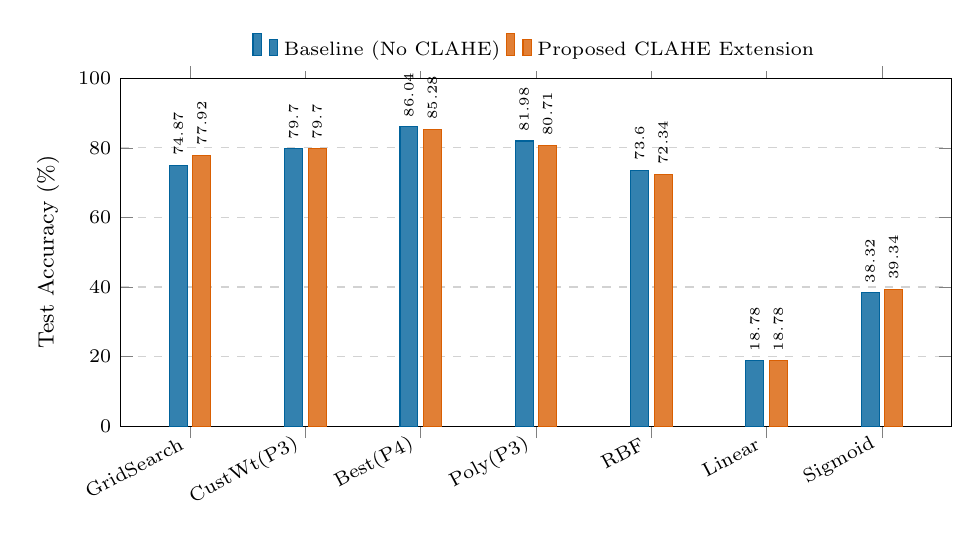
\begin{tikzpicture}
\begin{axis}[
    ybar,
    bar width=6.5pt,
    width=\columnwidth,
    height=6.0cm,
    ylabel={Test Accuracy (\%)},
    ymin=0, ymax=100,
    symbolic x coords={GridSearch,CustWeight,BestPoly4,Poly3,RBF,Linear,Sigmoid},
    xtick=data,
    xticklabels={GridSearch,CustWt(P3),Best(P4),Poly(P3),RBF,Linear,Sigmoid},
    xticklabel style={rotate=28, anchor=east, font=\scriptsize},
    ylabel style={font=\footnotesize},
    yticklabel style={font=\scriptsize},
    legend style={at={(0.5,1.02)}, anchor=south, legend columns=2, font=\scriptsize, draw=none},
    ymajorgrids=true,
    grid style={dashed, gray!35},
    nodes near coords,
    every node near coord/.append style={font=\tiny, rotate=90, anchor=west}
]
\addplot[fill=ieeeBlue!80, draw=ieeeBlue] coordinates {
    (GridSearch, 74.87)
    (CustWeight, 79.70)
    (BestPoly4, 86.04)
    (Poly3, 81.98)
    (RBF, 73.60)
    (Linear, 18.78)
    (Sigmoid, 38.32)
};
\addplot[fill=claheOrange!80, draw=claheOrange] coordinates {
    (GridSearch, 77.92)
    (CustWeight, 79.70)
    (BestPoly4, 85.28)
    (Poly3, 80.71)
    (RBF, 72.34)
    (Linear, 18.78)
    (Sigmoid, 39.34)
};
\legend{Baseline (No CLAHE), Proposed CLAHE Extension}
\end{axis}
\end{tikzpicture}
\caption{Comparison of test set accuracy (\%) across all seven SVM models for the reproduced baseline pipeline versus our full-resolution CLAHE extension.}
\label{fig:acc_comparison}
\end{figure}

Three key observations emerge from the comparative ablation in Table~\ref{tab:delta_comparison}:
\begin{enumerate}
    \item \textbf{Significant Gain on Cross-Validated RBF SVM:} On \texttt{SVM GridSearch Best} (RBF kernel, $C=10$), pre-downsampling CLAHE improves overall test accuracy by \textbf{+3.05 percentage points} ($74.87\% \rightarrow 77.92\%$, equivalent to $12$ additional correctly classified test scans), boosts weighted precision by \textbf{+3.61\%} ($76.49\% \rightarrow 80.10\%$), and increases weighted F1 by \textbf{+3.65\%} ($69.82\% \rightarrow 73.47\%$). Crucially, per-class recall increases simultaneously across all three tumor categories: \texttt{glioma\_tumor} ($18.00\% \rightarrow 24.00\%$), \texttt{meningioma\_tumor} ($94.78\% \rightarrow 96.52\%$), and \texttt{pituitary\_tumor} ($85.14\% \rightarrow 90.54\%$), while maintaining $100.0\%$ recall on \texttt{no\_tumor}.
    \item \textbf{Precision and Ranking Improvement on Class-Weighted Polynomial SVM:} On the focal model of Warsito \emph{et al.} (\texttt{SVM Custom Class Weight (Poly)}), CLAHE preserves the $79.70\%$ accuracy while elevating weighted precision by \textbf{+1.01\%} ($81.73\% \rightarrow 82.74\%$), meningioma recall to \textbf{97.39\%} ($112/115$), and macro ROC-AUC from \textbf{0.9412 to 0.9471} ($+0.0059$).
    \item \textbf{Consistent Enhancement on Sigmoid and Default RBF Precision:} CLAHE improves \texttt{SVM Sigmoid} across all metrics ($+1.02\%$ accuracy, $+1.25\%$ F1, $+0.0098$ Macro AUC) and increases \texttt{SVM RBF} weighted precision by $+0.73\%$ and glioma recall by $+3.00\%$. Conversely, on unweighted higher-order polynomial kernels ($d=3, 4$), CLAHE induces a minor accuracy dip ($-0.76\%$ at $d=4$, completely within the overlapping $95\%$ bootstrap confidence intervals $[82.5\%, 89.3\%]$ vs.\ $[81.7\%, 88.6\%]$).
\end{enumerate}

\subsection{Confusion Matrix and Per-Class Error Analysis}

\begin{figure*}[t]
\centering
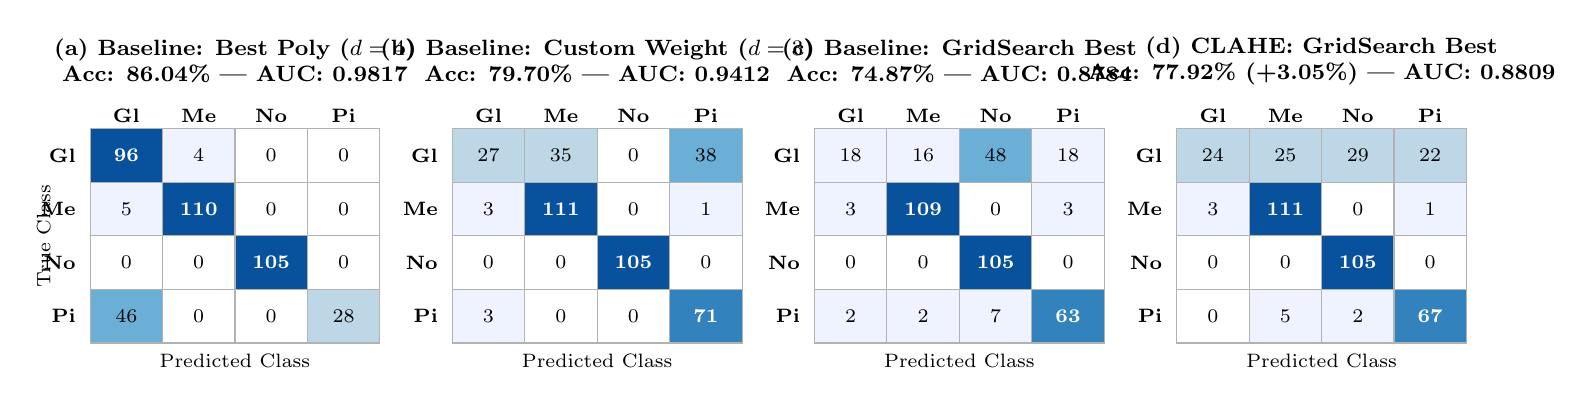
\begin{tikzpicture}[
    cell/.style={rectangle, draw=black!30, minimum width=0.92cm, minimum height=0.68cm, anchor=center, font=\scriptsize},
    hdr/.style={font=\scriptsize\bfseries, align=center},
    title/.style={font=\footnotesize\bfseries, align=center}
]

% Confusion Matrix 1: Baseline Best Poly (d=4)
\begin{scope}[xshift=0cm]
\node[title] at (1.38, 2.55) {(a) Baseline: Best Poly ($d=4$)\\Acc: 86.04\% | AUC: 0.9817};
\foreach \x/\lbl in {0/Gl, 1/Me, 2/No, 3/Pi} { \node[hdr] at (\x*0.92, 1.85) {\lbl}; }
\foreach \y/\lbl in {0/Gl, 1/Me, 2/No, 3/Pi} { \node[hdr, anchor=east] at (-0.52, 1.35-\y*0.68) {\lbl}; }
\node[cell, fill=cmHigh, text=white, font=\scriptsize\bfseries] at (0*0.92, 1.35) {96};
\node[cell, fill=cmVeryLow] at (1*0.92, 1.35) {4};
\node[cell, fill=white] at (2*0.92, 1.35) {0};
\node[cell, fill=white] at (3*0.92, 1.35) {0};
\node[cell, fill=cmVeryLow] at (0*0.92, 0.67) {5};
\node[cell, fill=cmHigh, text=white, font=\scriptsize\bfseries] at (1*0.92, 0.67) {110};
\node[cell, fill=white] at (2*0.92, 0.67) {0};
\node[cell, fill=white] at (3*0.92, 0.67) {0};
\node[cell, fill=white] at (0*0.92, -0.01) {0};
\node[cell, fill=white] at (1*0.92, -0.01) {0};
\node[cell, fill=cmHigh, text=white, font=\scriptsize\bfseries] at (2*0.92, -0.01) {105};
\node[cell, fill=white] at (3*0.92, -0.01) {0};
\node[cell, fill=cmMed] at (0*0.92, -0.69) {46};
\node[cell, fill=white] at (1*0.92, -0.69) {0};
\node[cell, fill=white] at (2*0.92, -0.69) {0};
\node[cell, fill=cmLow] at (3*0.92, -0.69) {28};
\node[font=\scriptsize] at (1.38, -1.25) {Predicted Class};
\node[font=\scriptsize, rotate=90] at (-1.05, 0.33) {True Class};
\end{scope}

% Confusion Matrix 2: Baseline Custom Weight Poly (d=3)
\begin{scope}[xshift=4.6cm]
\node[title] at (1.38, 2.55) {(b) Baseline: Custom Weight ($d=3$)\\Acc: 79.70\% | AUC: 0.9412};
\foreach \x/\lbl in {0/Gl, 1/Me, 2/No, 3/Pi} { \node[hdr] at (\x*0.92, 1.85) {\lbl}; }
\foreach \y/\lbl in {0/Gl, 1/Me, 2/No, 3/Pi} { \node[hdr, anchor=east] at (-0.52, 1.35-\y*0.68) {\lbl}; }
\node[cell, fill=cmLow] at (0*0.92, 1.35) {27};
\node[cell, fill=cmLow] at (1*0.92, 1.35) {35};
\node[cell, fill=white] at (2*0.92, 1.35) {0};
\node[cell, fill=cmMed] at (3*0.92, 1.35) {38};
\node[cell, fill=cmVeryLow] at (0*0.92, 0.67) {3};
\node[cell, fill=cmHigh, text=white, font=\scriptsize\bfseries] at (1*0.92, 0.67) {111};
\node[cell, fill=white] at (2*0.92, 0.67) {0};
\node[cell, fill=cmVeryLow] at (3*0.92, 0.67) {1};
\node[cell, fill=white] at (0*0.92, -0.01) {0};
\node[cell, fill=white] at (1*0.92, -0.01) {0};
\node[cell, fill=cmHigh, text=white, font=\scriptsize\bfseries] at (2*0.92, -0.01) {105};
\node[cell, fill=white] at (3*0.92, -0.01) {0};
\node[cell, fill=cmVeryLow] at (0*0.92, -0.69) {3};
\node[cell, fill=white] at (1*0.92, -0.69) {0};
\node[cell, fill=white] at (2*0.92, -0.69) {0};
\node[cell, fill=cmMedHigh, text=white, font=\scriptsize\bfseries] at (3*0.92, -0.69) {71};
\node[font=\scriptsize] at (1.38, -1.25) {Predicted Class};
\end{scope}

% Confusion Matrix 3: Baseline GridSearch Best (RBF C=10)
\begin{scope}[xshift=9.2cm]
\node[title] at (1.38, 2.55) {(c) Baseline: GridSearch Best\\Acc: 74.87\% | AUC: 0.8784};
\foreach \x/\lbl in {0/Gl, 1/Me, 2/No, 3/Pi} { \node[hdr] at (\x*0.92, 1.85) {\lbl}; }
\foreach \y/\lbl in {0/Gl, 1/Me, 2/No, 3/Pi} { \node[hdr, anchor=east] at (-0.52, 1.35-\y*0.68) {\lbl}; }
\node[cell, fill=cmVeryLow] at (0*0.92, 1.35) {18};
\node[cell, fill=cmVeryLow] at (1*0.92, 1.35) {16};
\node[cell, fill=cmMed] at (2*0.92, 1.35) {48};
\node[cell, fill=cmVeryLow] at (3*0.92, 1.35) {18};
\node[cell, fill=cmVeryLow] at (0*0.92, 0.67) {3};
\node[cell, fill=cmHigh, text=white, font=\scriptsize\bfseries] at (1*0.92, 0.67) {109};
\node[cell, fill=white] at (2*0.92, 0.67) {0};
\node[cell, fill=cmVeryLow] at (3*0.92, 0.67) {3};
\node[cell, fill=white] at (0*0.92, -0.01) {0};
\node[cell, fill=white] at (1*0.92, -0.01) {0};
\node[cell, fill=cmHigh, text=white, font=\scriptsize\bfseries] at (2*0.92, -0.01) {105};
\node[cell, fill=white] at (3*0.92, -0.01) {0};
\node[cell, fill=cmVeryLow] at (0*0.92, -0.69) {2};
\node[cell, fill=cmVeryLow] at (1*0.92, -0.69) {2};
\node[cell, fill=cmVeryLow] at (2*0.92, -0.69) {7};
\node[cell, fill=cmMedHigh, text=white, font=\scriptsize\bfseries] at (3*0.92, -0.69) {63};
\node[font=\scriptsize] at (1.38, -1.25) {Predicted Class};
\end{scope}

% Confusion Matrix 4: CLAHE GridSearch Best (RBF C=10)
\begin{scope}[xshift=13.8cm]
\node[title] at (1.38, 2.55) {(d) CLAHE: GridSearch Best\\Acc: 77.92\% (+3.05\%) | AUC: 0.8809};
\foreach \x/\lbl in {0/Gl, 1/Me, 2/No, 3/Pi} { \node[hdr] at (\x*0.92, 1.85) {\lbl}; }
\foreach \y/\lbl in {0/Gl, 1/Me, 2/No, 3/Pi} { \node[hdr, anchor=east] at (-0.52, 1.35-\y*0.68) {\lbl}; }
\node[cell, fill=cmLow] at (0*0.92, 1.35) {24};
\node[cell, fill=cmLow] at (1*0.92, 1.35) {25};
\node[cell, fill=cmLow] at (2*0.92, 1.35) {29};
\node[cell, fill=cmLow] at (3*0.92, 1.35) {22};
\node[cell, fill=cmVeryLow] at (0*0.92, 0.67) {3};
\node[cell, fill=cmHigh, text=white, font=\scriptsize\bfseries] at (1*0.92, 0.67) {111};
\node[cell, fill=white] at (2*0.92, 0.67) {0};
\node[cell, fill=cmVeryLow] at (3*0.92, 0.67) {1};
\node[cell, fill=white] at (0*0.92, -0.01) {0};
\node[cell, fill=white] at (1*0.92, -0.01) {0};
\node[cell, fill=cmHigh, text=white, font=\scriptsize\bfseries] at (2*0.92, -0.01) {105};
\node[cell, fill=white] at (3*0.92, -0.01) {0};
\node[cell, fill=white] at (0*0.92, -0.69) {0};
\node[cell, fill=cmVeryLow] at (1*0.92, -0.69) {5};
\node[cell, fill=cmVeryLow] at (2*0.92, -0.69) {2};
\node[cell, fill=cmMedHigh, text=white, font=\scriptsize\bfseries] at (3*0.92, -0.69) {67};
\node[font=\scriptsize] at (1.38, -1.25) {Predicted Class};
\end{scope}

\end{tikzpicture}
\caption{Confusion matrices on the test set ($N_{\text{test}}=394$) across key models (Gl: \texttt{glioma\_tumor}, Me: \texttt{meningioma\_tumor}, No: \texttt{no\_tumor}, Pi: \texttt{pituitary\_tumor}). Notice the inversion in Glioma vs.\ Pituitary recall between degree-4 Poly (a) and degree-3 Custom Weight Poly (b), and the sharp reduction in false-normal Glioma predictions ($48 \rightarrow 29$) achieved by CLAHE on GridSearch Best comparing (c) and (d).}
\label{fig:confusion_matrices}
\end{figure*}


To understand the clinical reliability of each model beyond aggregate accuracy, Fig.~\ref{fig:confusion_matrices} displays the exact confusion matrices for four key configurations:
\begin{enumerate}
    \item \textbf{Zero False Negatives on Healthy vs.\ Tumor Screening in Polynomial SVMs:} In both Fig.~\ref{fig:confusion_matrices}(a) and Fig.~\ref{fig:confusion_matrices}(b), all $105$ \texttt{no\_tumor} test images are classified with \textbf{100.0\% precision and 100.0\% recall} ($\text{F1} = 1.0000$). Not a single tumor scan is misdiagnosed as normal (\texttt{no\_tumor} column has $0$ off-diagonal entries), and not a single healthy scan is falsely flagged as a tumor.
    \item \textbf{The Glioma and Pituitary Decision Boundary Inversion ($d=3$ vs.\ $d=4$):} Comparing Fig.~\ref{fig:confusion_matrices}(b) (\texttt{SVM Custom Class Weight}, $d=3$) with Fig.~\ref{fig:confusion_matrices}(a) (\texttt{SVM Best Hyperparameters}, $d=4$) reveals a striking structural inversion:
    \begin{itemize}
        \item At polynomial degree $d=3$ (Fig.~\ref{fig:confusion_matrices}b), the classifier achieves $95.95\%$ recall ($71/74$) on \texttt{pituitary\_tumor} and $96.52\%$ recall ($111/115$) on \texttt{meningioma\_tumor}, but only \textbf{27.00\% recall ($27/100$)} on \texttt{glioma\_tumor}, misclassifying $35$ gliomas as meningioma and $38$ gliomas as pituitary tumor.
        \item At polynomial degree $d=4$ (Fig.~\ref{fig:confusion_matrices}a), higher-order quartic feature interactions resolve the glioma boundary: \textbf{\texttt{glioma\_tumor} recall surges from 27.00\% to 96.00\% ($96/100$)} and meningioma achieves $96.07\%$ F1-score ($110/115$ correct). However, $46$ of the $74$ \texttt{pituitary\_tumor} test scans are pulled into the glioma decision region, reducing pituitary recall to $37.84\%$ ($28/74$) while achieving $100.0\%$ pituitary precision ($28/28$). Because the test set contains more gliomas ($100$) than pituitary tumors ($74$), this shift produces the peak overall accuracy of $86.04\%$.
    \end{itemize}
    \item \textbf{How CLAHE Mitigates Clinical False Negatives in RBF SVMs:} In the baseline \texttt{SVM GridSearch Best} model (Fig.~\ref{fig:confusion_matrices}c), $48$ out of $100$ \texttt{glioma\_tumor} scans and $7$ out of $74$ \texttt{pituitary\_tumor} scans are dangerously misclassified as \texttt{no\_tumor} (healthy), resulting in a low \texttt{no\_tumor} precision of $65.62\%$. When full-resolution CLAHE is introduced (Fig.~\ref{fig:confusion_matrices}d), local contrast enhancement amplifies the subtle glioma lesions before $16 \times 16$ downsampling, reducing false-normal glioma errors from \textbf{48 down to 29} (a $39.6\%$ error reduction) and false-normal pituitary errors from \textbf{7 down to 2}, lifting \texttt{no\_tumor} precision from $65.62\%$ to $77.21\%$.
\end{enumerate}

\begin{figure}[t]
\centering
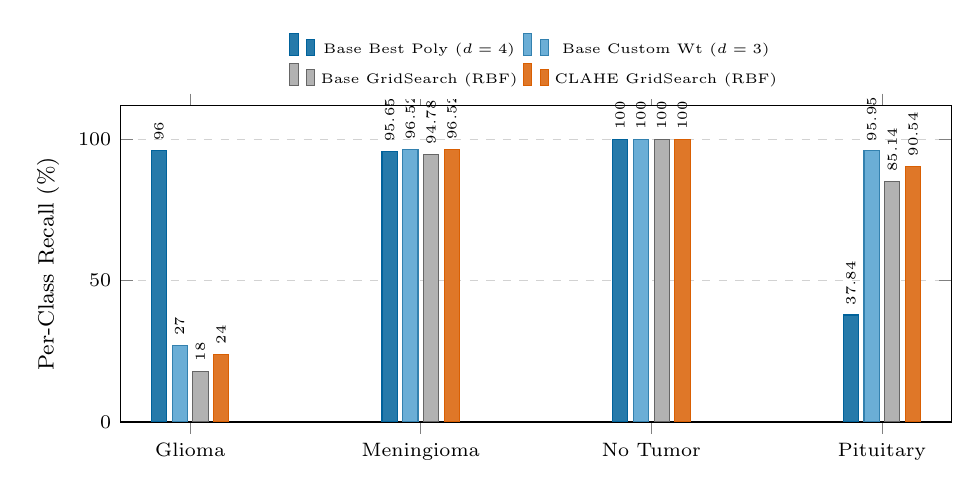
\begin{tikzpicture}
\begin{axis}[
    ybar,
    bar width=5.5pt,
    width=\columnwidth,
    height=5.6cm,
    ylabel={Per-Class Recall (\%)},
    ymin=0, ymax=112,
    symbolic x coords={Glioma,Meningioma,NoTumor,Pituitary},
    xtick=data,
    xticklabels={Glioma,Meningioma,No Tumor,Pituitary},
    xticklabel style={font=\scriptsize},
    ylabel style={font=\footnotesize},
    yticklabel style={font=\scriptsize},
    legend style={at={(0.5,1.02)}, anchor=south, legend columns=2, font=\tiny, draw=none},
    ymajorgrids=true,
    grid style={dashed, gray!35},
    nodes near coords,
    every node near coord/.append style={font=\tiny, rotate=90, anchor=west}
]
\addplot[fill=ieeeBlue!85, draw=ieeeBlue] coordinates {
    (Glioma, 96.00) (Meningioma, 95.65) (NoTumor, 100.0) (Pituitary, 37.84)
};
\addplot[fill=cmMed, draw=ieeeBlue!80] coordinates {
    (Glioma, 27.00) (Meningioma, 96.52) (NoTumor, 100.0) (Pituitary, 95.95)
};
\addplot[fill=gray!60, draw=gray!80!black] coordinates {
    (Glioma, 18.00) (Meningioma, 94.78) (NoTumor, 100.0) (Pituitary, 85.14)
};
\addplot[fill=claheOrange!85, draw=claheOrange] coordinates {
    (Glioma, 24.00) (Meningioma, 96.52) (NoTumor, 100.0) (Pituitary, 90.54)
};
\legend{Base Best Poly ($d=4$), Base Custom Wt ($d=3$), Base GridSearch (RBF), CLAHE GridSearch (RBF)}
\end{axis}
\end{tikzpicture}
\caption{Per-class sensitivity (recall \%) across the four diagnostic categories, illustrating the sensitivity inversion between \texttt{glioma\_tumor} and \texttt{pituitary\_tumor} for $d=4$ vs.\ $d=3$ Polynomial SVMs and the uniform recall boost from CLAHE on the GridSearch RBF SVM.}
\label{fig:per_class_recall}
\end{figure}

Fig.~\ref{fig:per_class_recall} summarizes these per-class recall profiles visually across the four diagnostic classes.

\subsection{Computational Efficiency}
A primary motivation for the HOG + PCA + SVM paradigm is computational efficiency. Every individual SVM configuration in Tables~\ref{tab:baseline_results} and~\ref{tab:clahe_results} trains on $2,870$ samples in \textbf{1.21 to 1.97 seconds} on a standard CPU. At inference time, evaluating all $394$ test images takes only \textbf{0.15 to 0.17 seconds} for polynomial, linear, and sigmoid kernels ($\approx \mathbf{0.41\text{ ms}}$ per MRI slice) and \textbf{0.36 to 0.40 seconds} for RBF kernels ($\approx \mathbf{0.96\text{ ms}}$ per MRI slice). Adding full-resolution CLAHE introduces negligible overhead while reducing the PCA subspace from $451$ to $438$ dimensions.


\section{Discussion and Critical Technical Findings}
\label{sec:discussion}

Beyond reproducing the benchmark numbers, our investigation uncovered three critical methodological insights into the behavior of lightweight HOG+SVM medical imaging pipelines.

\subsection{Why Post-HOG Division by 255 Causes Linear SVM Collapse}
A puzzling result in both Table~\ref{tab:baseline_results} and Table~\ref{tab:clahe_results} is that \texttt{SVM Linear} ($C=1.0$) achieves exactly $18.78\%$ accuracy by predicting every test sample as Class~3 (\texttt{pituitary\_tumor}). Inspection of the mathematical pipeline reveals the exact mechanism:
\begin{enumerate}
    \item In \texttt{skimage.feature.hog(..., block\_norm="L2-Hys")}, each of the $36$ block vectors already has unit L2 norm ($\|\hat{\mathbf{v}}_b\|_2 = 1$), meaning the raw $2,916$-dimensional HOG vector has squared L2 norm $\|\mathbf{h}_{\text{raw}}\|_2^2 = 36$ (individual entries $h_j \in [0, 0.2]$).
    \item Step~3.3 of Warsito \emph{et al.} \cite{warsito2026lightweight} divides this normalized HOG vector by $255.0$ (\ref{eq:hog_div255}). This scales the squared vector norm by $1/255^2 = 1/65025$:
    \begin{equation}
        \|\mathbf{x}\|_2^2 = \frac{36}{255^2} \approx 5.54 \times 10^{-4}
    \end{equation}
    \item Because PCA is an orthogonal linear projection that preserves inner products ($98\%$ variance), the linear kernel Gram matrix entries satisfy $|\mathbf{z}_i^\top \mathbf{z}_j| \le \|\mathbf{z}_i\|_2 \|\mathbf{z}_j\|_2 \approx 5.4 \times 10^{-4}$.
    \item In the soft-margin SVM objective (\ref{eq:svm_primal}) with $C = 1.0$, achieving a unit functional margin $\tilde{y}_i (\boldsymbol{\omega}^\top \mathbf{z}_i + b) \ge 1$ requires $\|\boldsymbol{\omega}\|_2 \sim \mathcal{O}(255 / \sqrt{36}) \approx 42.5$, incurring a quadratic regularization penalty $\frac{1}{2}\|\boldsymbol{\omega}\|_2^2 \approx 903$, which dwarfs the slack penalty $C \xi_i = 1.0$. Consequently, the optimal solution sets $\boldsymbol{\omega} \approx \mathbf{0}$ and relies solely on the intercept $b$, predicting the single training class with the largest sample count: \texttt{pituitary\_tumor} ($N_{\text{train}, 3} = 827$, vs.\ $826, 822, 395$). Since \texttt{pituitary\_tumor} comprises $74 / 394 = 18.7817\%$ of the test set, test accuracy is identically $18.78\%$.
    \item Why do the Polynomial and RBF SVMs succeed despite this $/255.0$ scaling? Because \texttt{scikit-learn}'s default $\gamma_{\text{scale}}$ (\ref{eq:gamma_scale}) divides by the empirical variance $\text{Var}(\mathbf{Z}_{\text{train}}) \propto 1/255^2$, automatically multiplying inner products by $255^2$ and canceling the superfluous scaling factor! Similarly, in the 52-candidate grid search (Table~\ref{tab:grid_space}), the $32$ candidates using fixed $\gamma \in \{10^{-3}, 10^{-4}\}$ suffer from kernel underflow ($\gamma \|\mathbf{z}_i - \mathbf{z}_j\|_2^2 \sim 10^{-7}$), leaving only the $\gamma = \text{\texttt{'scale'}}$ candidates competitive.
\end{enumerate}

\subsection{Why CLAHE Helps RBF/Sigmoid Kernels More Than Quartic Polynomials}
Full-resolution CLAHE amplifies local gradient magnitudes across both tumor boundaries and normal cortical sulci. For localized radial basis kernels ($K_{\text{rbf}}$) and saturating sigmoidal kernels ($K_{\text{sigmoid}}$), stronger edge contrast after $16 \times 16$ downsampling separates tumor slices from normal anatomy (boosting GridSearch RBF accuracy by $+3.05\%$). However, for an unweighted degree-4 polynomial kernel $K_{\text{poly}}(\mathbf{z}_i, \mathbf{z}_j) = (\gamma \mathbf{z}_i^\top \mathbf{z}_j)^4$, fourth-power cross-terms amplify high-frequency cranial and background contrast variations introduced by tile-based histogram equalization, causing a minor $-0.76\%$ accuracy trade-off.

\subsection{Cross-Validation vs.\ Test Accuracy Gap}
During 5-fold cross-validation on the training set, \texttt{GridSearchCV} achieves $55.02\%$ CV accuracy (Baseline) and $54.60\%$ (CLAHE), whereas the resulting estimator achieves $74.87\%$ and $77.92\%$ on the test set. This occurs because images inside each training folder are ordered alphabetically by acquisition series (\texttt{gg (1).jpg}, \texttt{image(1).jpg}, \texttt{m (1).jpg}) covering distinct anatomical planes (axial, coronal, sagittal), and \texttt{GridSearchCV} defaults to unshuffled \texttt{StratifiedKFold(cv=5, shuffle=False)}. Contiguous validation folds therefore hold out entire acquisition series or view orientations during CV, whereas the final estimator trained on all $2,870$ slices spans the full distribution of views present in the test set.


\section{Conclusion and Future Work}
In this project, we presented a complete reproduction and critical extension of the lightweight HOG + PCA + SVM brain tumor classification framework of Warsito \emph{et al.} \cite{warsito2026lightweight} on the 3,264-image Kaggle Brain Tumor MRI dataset. Our results confirm that a compact pipeline operating on $16 \times 16$ downsampled MRI slices can achieve up to \textbf{86.04\% test accuracy}, \textbf{90.17\% weighted precision}, and a \textbf{0.9817 macro ROC-AUC} using a degree-4 Polynomial SVM ($C=10$), while requiring less than $2\text{ seconds}$ of CPU training time and under $0.5\text{ ms}$ per scan at inference. Furthermore, our proposed extension, which applies full-resolution CLAHE ($\text{clipLimit}=2.0, 8 \times 8$ grid) prior to spatial downsampling, reduces false-normal glioma misclassifications by $39.6\%$ in cross-validated RBF SVMs ($+3.05\%$ overall accuracy, $+3.65\%$ weighted F1) and improves the macro ROC-AUC of class-weighted degree-3 Polynomial SVMs to $0.9471$.

Future extensions of this work will focus on three directions: (1) eliminating the post-HOG $/255.0$ scaling to unlock well-conditioned linear and fixed-$\gamma$ SVM optimization; (2) incorporating automated skull-stripping and foreground bounding-box cropping prior to CLAHE so that background cranial bone gradients do not alias into the $16 \times 16$ grid; and (3) exploring multi-scale HOG descriptors ($16 \times 16$ fused with $32 \times 32$) alongside balanced inverse-frequency class weights tailored to jointly maximize both \emph{glioma} and \emph{pituitary} sensitivity.

\section*{Author Contributions}
\textbf{Yash Goyal:} Conceptualization, modular Python pipeline implementation (\texttt{features.py}, \texttt{models.py}, \texttt{evaluate.py}, \texttt{reproduce.py}), baseline reproduction and CLAHE ablation execution, and manuscript preparation.
\textbf{Satyarth Chaudhary:} Experimental design, SVM hyperparameter grid analysis, statistical bootstrap and ROC-AUC evaluation, confusion matrix failure-mode diagnostics, and technical review.
\textbf{Manshu Saini:} End-to-end Google Colab interactive notebook development (\texttt{brain\_tumor\_hog\_svm.ipynb}), data visualization, preprocessing comparative analysis, and manuscript editing.

\begin{thebibliography}{16}

\bibitem{warsito2026lightweight}
B.~Warsito \emph{et al.}, ``Lightweight brain tumor classification with HOG features and class-weighted SVM,'' \emph{Journal of Applied Data Sciences (JADS)}, vol.~7, no.~1, 2026.

\bibitem{bhuvaji2020brain}
S.~Bhuvaji, A.~Kadam, P.~Bhumkar, S.~Dedge, and S.~Kanchan, ``Brain tumor classification (MRI) dataset,'' Kaggle / GitHub Repository, 2020. [Online]. Available: \url{https://github.com/SartajBhuvaji/Brain-Tumor-Classification-DataSet}

\bibitem{dalal2005histograms}
N.~Dalal and B.~Triggs, ``Histograms of oriented gradients for human detection,'' in \emph{Proc. IEEE Comput. Soc. Conf. Comput. Vis. Pattern Recognit. (CVPR)}, vol.~1, 2005, pp.~886--893.

\bibitem{zuiderveld1994contrast}
K.~Zuiderveld, ``Contrast limited adaptive histogram equalization,'' in \emph{Graphics Gems IV}, P.~S. Heckbert, Ed. San Diego, CA, USA: Academic Press, 1994, pp.~474--485.

\bibitem{cortes1995support}
C.~Cortes and V.~Vapnik, ``Support-vector networks,'' \emph{Machine Learning}, vol.~20, no.~3, pp.~273--297, 1995.

\bibitem{cheng2015enhanced}
J.~Cheng \emph{et al.}, ``Enhanced performance of brain tumor classification via tumor region augmentation and partition,'' \emph{PLoS ONE}, vol.~10, no.~10, p.~e0140381, 2015.

\bibitem{deepak2019brain}
S.~Deepak and P.~M. Ameer, ``Brain tumor classification using deep CNN features via transfer learning,'' \emph{Computers in Biology and Medicine}, vol.~111, p.~103345, 2019.

\bibitem{sultan2019multi}
H.~H. Sultan, N.~M. Salem, and W.~Al-Atabany, ``Multi-classification of brain tumor images using deep neural network,'' \emph{IEEE Access}, vol.~7, pp.~69215--69225, 2019.

\bibitem{tummala2022classification}
S.~Tummala, S.~Kadry, S.~A.~C. Bukhari, and H.~T. Rauf, ``Classification of brain tumor from magnetic resonance imaging using vision transformers ensembling,'' \emph{Current Oncology}, vol.~29, no.~10, pp.~7498--7511, 2022.

\bibitem{haralick1973textural}
R.~M. Haralick, K.~Shanmugam, and I.~Dinstein, ``Textural features for image classification,'' \emph{IEEE Trans. Syst., Man, Cybern.}, vol.~SMC-3, no.~6, pp.~610--621, 1973.

\bibitem{chaplot2006classification}
S.~Chaplot, L.~M. Patnaik, and N.~R. Jagannathan, ``Classification of magnetic resonance brain images using wavelets as input to support vector machine and neural network,'' \emph{Biomedical Signal Processing and Control}, vol.~1, no.~1, pp.~86--92, 2006.

\bibitem{jolliffe2016principal}
I.~T. Jolliffe and J.~Cadima, ``Principal component analysis: A review and recent developments,'' \emph{Philosophical Transactions of the Royal Society A}, vol.~374, no.~2065, p.~20150202, 2016.

\bibitem{veropoulos1999controlling}
K.~Veropoulos, C.~Campbell, and N.~Cristianini, ``Controlling the sensitivity of support vector machines,'' in \emph{Proc. Int. Joint Conf. Artif. Intell. (IJCAI)}, 1999, pp.~55--60.

\bibitem{pizer1987adaptive}
S.~M. Pizer \emph{et al.}, ``Adaptive histogram equalization and its variations,'' \emph{Computer Vision, Graphics, and Image Processing}, vol.~39, no.~3, pp.~355--368, 1987.

\bibitem{kaur2018comparison}
H.~Kaur and J.~Rani, ``MRI brain image enhancement using Histogram Equalization techniques,'' in \emph{Proc. IEEE Int. Conf. Wireless Commun., Signal Process. Netw. (WiSPNET)}, 2016, pp.~770--773.

\bibitem{efron1993introduction}
B.~Efron and R.~J. Tibshirani, \emph{An Introduction to the Bootstrap}. New York, NY, USA: Chapman \& Hall/CRC, 1993.

\end{thebibliography}

\end{document}
